\section{Secondary Producer Service}\label{sec:SecondaryProducer}\index{secondary producer}

\subsection{Description}

Secondary Producer resources are created by the Secondary Producer
Service at the request of a user to
\textit{republish}\index{republish} one or more tables in a virtual
database. Republishing means running a ``SELECT * WHERE'' query
against a table in the virtual database and publishing the resulting
tuples back to the same table. The mediator ensures this isn't
recursive. As the picture below shows, the principal components of a
Secondary Producer are the same as a Primary Producer. All Secondary
Producers support continuous queries, and can be configured to support
any combination of latest and history queries as well.

\begin{center}
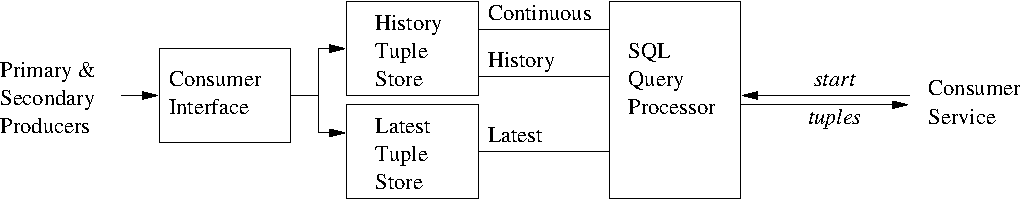
\includegraphics[width=160mm]{sp_detail}
\end{center}

The value of a Secondary Producer is that it creates real tables from
virtual ones, because it collects all tuples inserted into the virtual database
for any table it's republishing, into its own tuple stores. This means it can
act as an archiver for the tables, can answer queries involving joins between
them (even tables in different VDBs) because they're all in one database,
and can be used to reduce the load on other producers.

The Secondary Producer Service is responsible for authenticating all
users and services that connect to it, and for authorizing all
operations and all requests to access its tuple stores, as specified
in chapter \ref{sec:Security}.

\subsection{Interface}

\subsubsection{User Interface}

\begin{method}{createSecondaryProducer}
\inpar{xsd:boolean isHistory}{If history queries are supported}
\inpar{xsd:boolean isLatest}{If latest queries are supported}
\inpar{xsd:string type} {DATABASE or MEMORY}
\inpar{xsd:string logicalName}{The logical name should not be
be specified for type MEMORY. For type DATABASE it is optional.} 
\outhead{Tuple(1..1)}{}
\outpar{xsd:int connectionId}{connectionId of new Secondary Producer resource.} 
\desc Creates a new Secondary Producer resource and returns its endpoint. The
Secondary Producer is not added to a Registry until \textit{declareTable} is
called. The user cannot prevent Secondary Producers from supporting
continuous queries, but support for latest and/or history queries is optional.
Secondary Producers can use any type of storage, regardless of the query types
they support. Tuple stores can be made permanent by providing a
\textit{logical name} for the tuple store as described in
\ref{sec:SecondaryProducerTupleStores}.
The termination interval is described in \ref{sec:SecondaryProducerCreating}.
\end{method}

\begin{method}{declareTable}
\inpar{xsd:int connectionId}{Secondary Producer resource identifier.}
\inpar{xsd:string tableName}{VDBTable to register.}
\inpar{xsd:string predicate}{Producer's predicate.}
\inpar{xsd:int hrpSec}{History Retention Period in seconds.}
\OK
\desc
Adds a table to the list of tables republished by this producer, as described
in \ref{sec:SecondaryProducerDeclaring}. The table name must have an explicit
virtual database name prefix (separated from it by a dot).
The format of the
predicate is specified in \ref{sec:SQLPredicates}; by construction, a Secondary
Producer will republish \textit{all} tuples that match its predicate. The
retention period is described in \ref{sec:SecondaryProducerRemoving}.\\
\end{method}\par

\begin{method}{showSignOfLife}
\inpar{xsd:int connectionId}{Resource identifier.}
\OK
\desc Sends a sign-of-life request to a resource as a way to keep
the resource alive. Any other user operation on the resource will also serve
to keep it alive.
\end{method}

See also the common producer service operations:
getHistoryRetentionperiod~\ref{op:getHistoryRetentionPeriod}.

See also the common resource management service operations:
close~\ref{op:close} and destroy~\ref{op:destroy}.

See also the operations common to all services:
getProperty~\ref{op:getProperty}.

\subsubsection{System Interface}

\begin{method}{secondary}{addProducer}
\inpar{xsd:int connectionId}{Consumer resource identifier.}
\inpar{xsd:string url}{Producer URL.}
\inpar{xsd:int id}{Producer resource identifier.}
\inpar{xsd:string tableName}{Table name}
\inpar{xsd:string predicate}{Predicate}
\inpar{xsd:int hrpSec}{History Retention Period in seconds}
\inpar{xsd:boolean isHistory} {If producer supports history queries}
\inpar{xsd:boolean isLatest}{If producer supports latest queries}
\inpar{xsd:boolean isContinuous}{If producer supports continuous queries}
\inpar{xsd:boolean isStatic}{If producer supports static queries}
\inpar{xsd:boolean isSecondaryProducer}{If producer is secondary}
\inpar{xsd:string qosAttrib}{The QOS attribute - not used currently}
\OK
\desc Sent by a producer service to a continuous consumer or secondary producer
to notify it about an
addition to the list of relevant producers in the registry. Ignored if the
query is not currently executing. See the \textit{plan maintenance} section
(\ref{sec:ConsumerPlanMaintenance}) for how the consumer or secondary
producer should react to this.
\end{method}

\begin{method}{removeProducer}
\inpar{xsd:int connectionId}{Consumer resource identifier.}
\inpar{xsd:string url}{Producer URL.}
\inpar{xsd:int id}{Producer resource identifier.}
\OK
\end{method}

See  the common producer service operations:
start~\ref{op:start} and abort~\ref{op:producerabort}.

See the common resource management service operation:
ping~\ref{op:resourceping}.

\subsection{Details}
\subsubsection{Creating and destroying Secondary Producers}\label{sec:SecondaryProducerCreating}

A new Secondary Producer resource is created when a user calls the
\textit{createSecondaryProducer} operation and is destroyed when the user calls
the \textit{close} or \textit{destroy} operations. In addition,
if the service does not hear from the user for a period exceeding the
\textit{termination interval}, the service will initiate a \textit{close} operation
on the resource. A call to any user operation on the resource is sufficient
to keep it alive.

\subsubsection{Tuple stores}\label{sec:SecondaryProducerTupleStores}

These are exactly as in the Primary Producer Service (see
\ref{sec:PrimaryProducerTupleStores}) but System Administrators should
be even more wary of granting direct access to permanent tuple stores
maintained by Secondary Producers because Secondary Producers are granted
special access to the tuple stores of the producers from which they are
consuming, and those producers trust them to enforce the data access rules
of the VDB when republishing the data.

\subsubsection{Declaring tables (as a producer)}\label{sec:SecondaryProducerDeclaring}

The semantics of \textit{declareTable} are identical from the user's point of 
view to the Primary Producer, except that there is no Latest Retention Period 
to set. Internally, the service prepares the tuple stores then registers the 
Secondary Producer resource as a producer by calling 
\textit{registerProducerTable} and periodically calls this again to keep itself 
registered.

\subsubsection{Declaring tables (as a consumer)}\label{sec:ConsumerDeclaring}

Unlike a Primary Producer, the Secondary Producer must also act as a continuous
consumer for each declared table, by running a 
``SELECT * FROM \textit{tableName} WHERE \textit{predicate}'' query on the
virtual database. The procedure for identifying and notifying the producers
that will answer this query is exactly as in \ref{sec:ConsumerStarting} and
the list of producers is maintained as described in
\ref{sec:ConsumerPlanMaintenance}. A side effect of this is to register the
Secondary Producer resource as a \textit{secondary} consumer and keep it
registered. Flagging the resource as a secondary consumer simply allows
the mediator to ensure that it doesn't generate recursive query plans - in all
other respects, the mediator and the registry service treat the secondary
producer resource like any other continuous consumer and no further distinction
is made in this document. Likewise, the secondary producer presents the same
streaming interface to producers as described in
\ref{sec:ConsumerStreaming} for continuous consumers.

\subsubsection{Inserting tuples}\label{sec:SecondaryProducerInserting}
Tuples are inserted into a Secondary Producer by the service itself (by its 
streaming server). Users do not insert tuples into a Secondary Producer 
directly. Secondary Producers do not modify the tuples they store in any way.

\subsubsection{Removing tuples}\label{sec:SecondaryProducerRemoving}
The rules for History Retention Periods and Latest Retention Times in a
secondary producer are identical to a primary producer.

The \textit{close} call, however, is different from a primary producer. Since a
secondary producer must stop consuming immediately after a \textit{close}
request it must also stop servicing queries too, because it no longer holds a
complete set of tuples for the tables that it claims to republish.
Therefore \textit{close} means the same as \textit{destroy} in a secondary
producer.

\subsubsection{Processing queries}\label{sec:SecondaryProducerQueryProcessing}

Query processing in a Secondary Producer is identical to a Primary Producer
(see \ref{sec:PrimaryProducerQueryProcessing}).

\subsubsection{Stopping queries}\label{sec:SecondaryProducerStoppingQueries}

This is also identical to a Primary Producer
(see \ref{sec:PrimaryProducerStoppingQueries}).


